\documentclass[a4paper,11pt]{article}
\usepackage[english]{babel}
\usepackage[utf8]{inputenc}
\usepackage{graphicx} 
\usepackage{booktabs} 
\usepackage{algorithm}
\usepackage{framed}
\usepackage{tikz-cd}
%\usepackage{adjustbox}
%\usepackage{pst-node, auto-pst-pdf}


\usepackage[backslant]{aurical}       % Fontauri fonts 
\usepackage{bm}
\usepackage[utf8]{inputenc} % allow utf-8 input
%\usepackage[T1]{fontenc}    % use 8-bit T1 fonts
\usepackage{hyperref}       % hyperlinks
\usepackage{url}            % simple URL typesetting
\usepackage{booktabs}       % professional-quality tables
\usepackage{amsfonts}       % blackboard math symbols
\usepackage{nicefrac}       % compact symbols for 1/2, etc.
\usepackage{microtype}      % microtypography
\usepackage{subfig}
\usepackage{tabularx}
\usepackage{amsmath}
\usepackage{enumerate}
\usepackage{xcolor}
\usepackage[font=small]{caption}
%\usepackage[labelformat = empty,position=top]{subcaption}
\usepackage[export]{adjustbox}
%\usepackage{subcaption}

\usepackage[backend=biber,style=apa,sorting=ynt]{biblatex}

% \bibliographystyle{plainnat}

\usepackage{float}
\usepackage{placeins}
\usepackage{multirow}
\usepackage{mdframed}
\usepackage{media9}

\captionsetup[algorithm]{labelformat=empty}
% \usepackage{algpseudocode}
\usepackage{algorithmic}

\newcommand{\ols}{\textsc{ols}}


\newenvironment{itemize*}{
\begin{itemize}
\setlength{\parskip}{0em}
\setlength{\topparskip}{0em}
}
{\end{itemize}}

\newenvironment{enumerate*}{
\begin{enumerate}
\setlength{\parskip}{0em}
\setlength{\topparskip}{0em}
}
{\end{enumerate}}


% Commands
\newcommand{\comment}[1]{}
\newcommand{\techreport}[1]{#1}

\newcommand{\beq}{\begin{equation}}
\newcommand{\eeq}{\end{equation}}
\newcommand{\beqa}{\begin{eqnarray}}
\newcommand{\eeqa}{\end{eqnarray}}
\newcommand{\beqas}{\begin{eqnarray*}}
\newcommand{\eeqas}{\end{eqnarray*}}

\newcommand{\bit}{\begin{itemize}}
\newcommand{\eit}{\end{itemize}}
\newcommand{\bits}{\begin{itemize*}}
\newcommand{\eits}{\end{itemize*}}
\newcommand{\benum}{\begin{enumerate}}
\newcommand{\eenum}{\end{enumerate}}
\newcommand{\benums}{\begin{enumerate*}}
\newcommand{\eenums}{\end{enumerate*}}
\newcommand{\mybullet}{$\bullet$}

%\newcommand{\BlackBox}{\rule{1.5ex}{1.5ex}}  % end of proof

% names

\newcommand{\dpullalg}{{\sc PullBackDPhi}}
\newcommand{\projg}{{\sc ProjectG}}
\newcommand{\glassoalg}{{\sc GroupLasso}}
\newcommand{\embedalg}{{\sc EmbeddingAlg}}
\newcommand{\flassoalg}{{\sc GroupLasso}}
\newcommand{\flasso}{{\sc GroupLasso}}  % to be replaced with \flassoalg !!
\newcommand{\LEalg}{{\sc LaplacianEigenmaps}}
\newcommand{\rmalg}{{\sc RMetric}}
\newcommand{\lapalg}{{\sc Laplacian}}
\newcommand{\tppalg}{{\sc LocalPCA}}
\newcommand{\ouralg}{{\sc ManifoldLasso}}


\newcommand{\srdata}{{\bf SwissRoll}}
\newcommand{\redata}{{\bf RigidEthanol}}
\newcommand{\ethdata}{{\bf Ethanol}}
\newcommand{\toldata}{{\bf Toulene}}
\newcommand{\maldata}{{\bf Malonaldehyde}}

%  math mode commands

\newcommand {\argmax}[2]{\mbox{\raisebox{-1.7ex}{$\stackrel{\textstyle
 {\rm #1}}{\scriptstyle #2}$}}\,}
\newcommand{\nchoosem}[2]{\left(\!\!\!\begin{array}{c}#1\\#2\end{array}\!\!\!\right)}  % use \binom{}{} instead
\newcommand{\fracpartial}[2]{\frac{\partial #1}{\partial  #2}}

\newcommand{\bigOO}{{\cal O}}
\newcommand{\dataset}{{\cal D}}
\newcommand{\onevector}{{\mathbf 1}}
\newcommand{\rrr}{{\mathbb R}}

\newcommand{\M}{{\cal M}}
\newcommand{\T}{{\cal T}}
\newcommand{\txim}{\ensuremath{\T_{\xi_i}\M}} % tangent subspace
\newcommand{\I}{{\cal I}} % set of indices for which to compute gradients

\newcommand{\G}{{\cal G}} % dictionary
\newcommand{\neigh}{{\cal N}}
\newcommand{\X}{{\cal X}}
\newcommand{\xb}{\mathbf{X}}  % matrices for glasso
\newcommand{\tilx}{\tilde{x}}
%\newcommand{\g}{\Fontauri{g}} % R metric as a form Fontauri not working!
\newcommand{\g}{\mathbf{g}} % R metric as a form
%\newcommand{\id}{\Fontauri{id}} % induced Euclidean metric as a form
\newcommand{\id}{\mathbf{id}} % induced Euclidean metric as a form


\newcommand{\proj}{\operatorname{Proj}}
\newcommand{\trace}{\operatorname{trace}}
\newcommand{\rank}{\operatorname{rank}}
\newcommand{\range}{\operatorname{span}}
\newcommand{\rowrange}{\operatorname{rowspan}}
\newcommand{\diag}{\operatorname{diag}}
\newcommand{\grad}{\operatorname{grad}}
\newcommand{\supp}{\operatorname{supp}}

\newcommand{\barbx}{\bar{\bar{X}}}
\newcommand{\bhat}{\hat{\beta}}
\newcommand{\zhat}{\hat{z}}
\newcommand{\barw}{\bar{\epsilon}}
\newcommand{\bbar}{\bar{\beta}}

\newcommand{\E}{{\cal E}} %the error manifold
\newcommand{\N}{{\cal N}} %a normal space
\newcommand{\Ho}{{\cal H}} %the horizontal space of a map
\newcommand{\V}{{\cal V}} %the vertical space of a map
\newcommand{\B}{{\cal B}} %the base manifold
\newcommand{\txm}{\ensuremath{\T_{\xi}\M}}
\newcommand{\tbasis}{\mathbf{T}} % basis T
\newcommand{\cp}{\text{cp}}
\newcommand{\tstsbp}{{\sc TwoStageTSBP}}
\newcommand{\tsalg}{{\sc TSLasso}}
\newcommand{\tsbp}{{\sc TSBasisPursuit}}
\newcommand{\embedts}{\textsc{EmbedTS}}
\newcommand{\embedgrad}{{\sc EmbedGrad}}
\captionsetup[algorithm]{labelformat=empty}
\newtheorem{proposition}{Proposition}


\tikzset{%
  symbol/.style={
    draw=none,
    every to/.append style={
      edge node={node [sloped, allow upside down, auto=false]{$#1$}}
    },
  },
}

\usepackage{tcolorbox}

\tcbuselibrary{fitting}

\newenvironment{proof}{\paragraph{Proof:}}{\hfill$\square$}



\begin{document}

\title{Isometry pursuit}
\author{Samson Koelle, Marina Meila}

\maketitle

\begin{abstract}

Isometry pursuit is an algorithm for identifying unitary column-submatrices of wide matrices in polynomial time. % find citation for convexity implying polynomial time.  Tropp?
It achieves sparsity via use of the group lasso norm, and therefore has constrained and penalized formulations.
Applied to tabular data, it selects a subset of columns that maximize diversity.
Applied to Jacobians of putative coordinate functions, it identifies isometric embeddings from within dictionaries.
It therefore has relevance to interpretability of learned representations.

\end{abstract}

\section{Introduction}
\label{sec:introduction}

Many real-life problems may be abstracted as selecting a subset of the columns of a matrix representing stochastic observations or analytically exact data.
This paper focuses on a simple such problem that appears in unsupervised learning.
Given a rank $D$ matrix $\mathcal X \in \mathbb R^{D \times P}$ with $P > D$, select a square submatrix $\mathcal X_{.\mathcal S}$ where subset $\mathcal S \subset P$ satisfies $|\mathcal S| = D$ that is as unitary as possible.

This problem is motivated by applications in diversification and non-linear dimension reduction.
In particular, the name of the method comes from the fact that isometric embeddings have unitary differentials.
While variable selection in unsupervised learning is comparably less studied than in supervised learning, substantial literature exists.
One method that exemplifies this area is Sparse PCA \cite{Dey2017-mx}, in which a subset of variables are used to generate low-dimensional projections.
% compared with sparse pca loadings are constrained to be 1.  is it convex?
Within non-linear dimension reduction dictionaries can be either given \cite{Koelle2022-ju, Koelle2024-no} or learned \cite{Kohli2021-lr}. 
In order of specificity, these methods may seek to optimize independent coordinates \cite{Chen2019-km, He2023-ch}, low distortion embeddings, or isometric embeddings.
Optimization can be global or local.
These coordinate selection algorithms can be greedy \cite{NEURIPS2019_6a10bbd4, Kohli2021-lr, Jones2007-uc} or convex \cite{Koelle2022-ju, Koelle2024-no}.
%% cite sparse 
%Many of these operate locally.

%(RAG, recommendations, training neural networks (infrequent meta), wind).

The insight that leads to isometry pursuit is that $D$ function solutions multitask basis pursuit applied to an appropriately normalized $\mathcal X$ selects unitary submatrices.
%This approach relies on a to-our-knowledge novel matrix inversion algorithm that is sparse in the column space of the matrix.
This normalization is log-symmetric length in the column-space of $\mathcal X$ and favors vectors closer to unit length.
This property is the focus of Section \ref{sec:theory}

The basis pursuit formulation is desirable for several reasons.
First, it is convex and therefore computationally expedient.
Second, while not $D$-sparse, it is relatively sparse, and so can be used for pruning. % we need more theory on the D subset within the retained subset, need to compare brute force and trimmed solutions.
Third, it admits a lasso dual problem which is particularly useful in high dimensions.

%These problems are solvable with off-the-shelf multitask lasso and interior point solvers, respectively.
% Square selection could be relaxed somewhat.

%Unsupervised learning methods like PCA, UMAP, and autoencoders are often concerned with minimizing reconstruction error without regard for the sparsity of the learned respresentation, and among those that sparsify, variable selection methods contrast with sparsification with respect to reconstruction from a learned latent space.

% Multitask learning and lasso \cite{Hastie2015-qa}

%Within the context of non-linear dimension reduction, selection of coordinate functions of an embedding space from within a dictionary is a core problem in geometric data analysis.  % more on interpretability

%In this paper we show that an adapted version of the group lasso type algorithm in \cite{Koelle2024-no} leads to a convex procedure competitive with previous greedy approaches with respect to isometry.

% cite some classic manifold learning papers

%The comparison of greedy (e.g. Orthogonal Matching Pursuit) \cite{Mallat93-wi, Tropp05-ml} and convex \cite{Tropp06-sg} basis pursuit formulations.

%Basis pursuit \cite{Chen2001-hh} 
% Recommendation, RAG

\section{Background}

\subsection{Problem}

As mentioned in Section \ref{sec:introduction}, our goal is to select a subset $\mathcal S \subset [P]$ with $|\mathcal S| = D$ such that $X_{. \mathcal S}$ is as unitary as possible.
To that end, we must define what this means.

\subsection{Isometries}

\begin{definition}{Isometric at a point}
Two $D$ dimensional manifolds $\mathcal M$ and $\mathcal N$ are \textbf{isometric at a point} $p \in \mathcal M$ if
\begin{align}
u^T v = (D \phi (p) u)^T v \forall u,v \in \mathcal T_p \mathcal M
\end{align}
where $T_p \mathcal M$ is the tangent space of $\mathcal M$ at $p$.
\end{definition}

%Note that in the case of tabular data, where $\mathcal M = \mathbb R^P$, and $\mathcal N = \mathbb R^D$, and $\phi \in \mathbb R^{D \times P}$ is a linear map, this is equivalent to saying that $\phi$ is unitary.
$X$ could be, for example, the Jacobian matrix $d g$ of a set of candidate coordinate functions $g = [g^1, \dotsc g^P]$.

% We assume that we are given a target dimension $T \leq D$ - do we?
% BIG QUESTION: RUN IN D = B?  What is rank of $X$?    It's D if not running D = B

\section{Method}

% balance goes out the window with great flowers - no normalization.

\subsection{Normalization}

Since basis pursuit methods tend to select longer vectors, selection of unitary submatrices requires normalization such that long and short candidate basis vectors are penalized equivalently.
Thus, let
\begin{align}
\label{eq:normalization}
q: \mathbb R^+ \times \mathbb R^+  &\to \mathbb R^+ \\
t , c &\mapsto \frac{\exp(t^c) + \exp(t^{-c})}{2e},
\end{align}
and use this to define the normalization 
\begin{align}
n: \mathbb R^D \times \mathbb R^+ &\to \mathbb R^D \\
n^d , c &\mapsto \frac{n^d}{q(\|n\|_{2},c) } \forall d \in [D].
\end{align}

This normalization scales lengths down that are far away from $1$ is a logarithmically symmetric way.
Any rescaling which is maximized at $1$ and logarithmically symmetric satisfies Proposition \ref{prop:main}, but $n$ is particularly suitable.
First, $q$ is convex.
Second, it grows asymptotically log-linearly.
Third, while $\exp(-|\log t|) = \exp(-\max (t, 1/t))$ is a seemingly natural choice for normalization, it is non smooth, and the LogSumExp replacement of $\max (t, 1/t)$ with $ \log (\exp (t ) + \exp(1/t))$ simplifies to \ref{eq:normalization} upon the exponentiation.
Finally, the parameter $c$ grants control over the width of the basin, which is important in avoiding numerical issues arising close to $0$ and $\infty$.

\begin{figure}[htbp]
    \centering
    \begin{minipage}{0.49\textwidth}
        \centering
        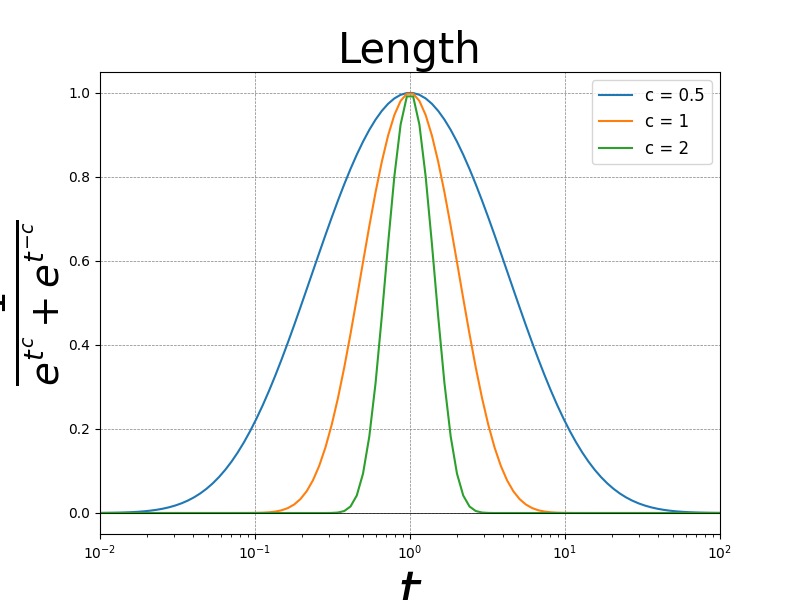
\includegraphics[width=\textwidth]{../figures/Figure_1a.png}
        \caption{Length as a function of $t$}
        \label{fig:length}
    \end{minipage}
    \hfill
    \begin{minipage}{0.49\textwidth}
        \centering
        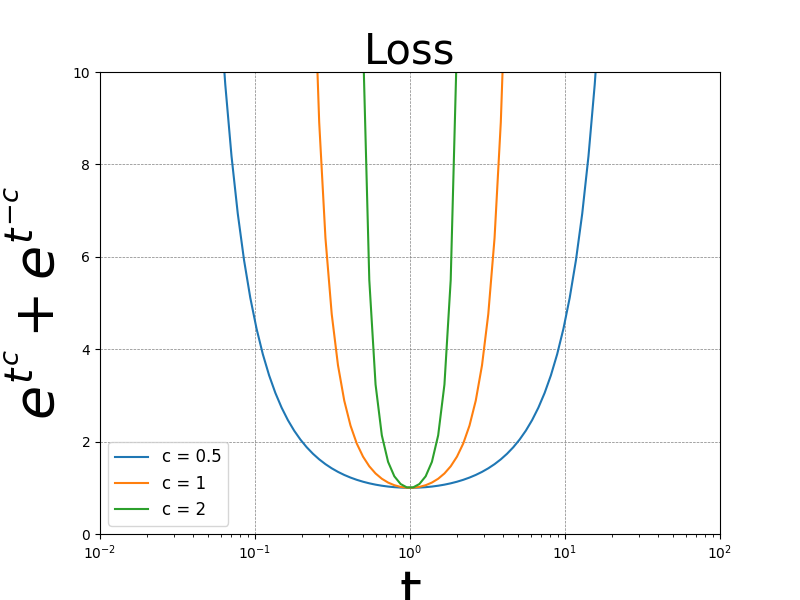
\includegraphics[width=\textwidth]{../figures/Figure_1b.png}
        \caption{Loss as a function of $t$}
        \label{fig:loss}
    \end{minipage}
    \caption{Plots of Length and Loss for different values of $c$}
    \label{fig:results}
\end{figure}


Using this, define the matrix-wide normalization vector
\begin{align}
\mathcal D: \mathbb R^{D \times P} \times \mathbb R^+ &\to \mathbb R^P \\
\mathcal X_{.p}, c &\mapsto n(\mathcal X_{.p}, c)
\end{align}
and the normalized matrix $\tilde {\mathcal X}_c = \mathcal X \mathcal D(\mathcal X, c).$
This completes the data preprocessing.

\subsection{Ground truth}

The main goal of sparse isometry pursuit is to expediate the selection of unitary submatrices.
Typically, unitaryness is measured using the singular values of the matrix.
However, measures like the operator norm and deformation compare only the largest an smallest singular values.
Compared with the nuclear norm, it is symmetric around 1 \cite{Fazel2001ARM}. % is our loss self-dual?
That is, they do not account for the whole spectrum.

Define the loss
\begin{align}
l_{iso}: \mathbb R^{D \times P} \to \mathbb R^{+} \\
\mathcal (X) \mapsto \sum_{d = 1}^D g(\sigma^d(\mathcal X))
\end{align}
where $\sigma^d (\mathcal (X))$ is the $d$-th singular value of $\mathcal X$.
%Note that since $g$ is convex, we could compute a full realization of the convex isometry pursuit algorithm by minimizing over WHAT.
However, this would not result in a sparse solution.

This loss is an appropriate choice for comparison because it is equal to the basis pursuit loss for orthogonal matrices
\begin{proposition}
\label{prop:main}
\end{proposition}
\begin{proof}
\begin{align}
\end{align}
Then, singular values and regressands are analytically determined.  cont.
\end{proof}

\subsection{Isometry pursuit}

Define the multitask group basis pursuit penalty % is this really a norm?
\begin{align}
\label{eq:bp}
\| \cdot \|_{1,2}: \mathbb R^{P \times D} &\to \mathbb R^+ \\ 
\beta &\mapsto  \sum_{p=1}^P  \|\beta_{p.}\|_2.
\end{align}

The isometry pursuit program is then
\begin{align}
\label{prog:isometry_pursuit}
\hat {\beta_{P}} (\mathcal X)  = \arg \min_{\beta \in \mathbb R^{P \times D}} \| \beta \|_{1,2} \; s.t. \; I_D = \tilde{ \mathcal X}_c \beta.
\end{align}
The intuition is that vectors which are closer to 1 in length and more orthogonal will be smaller in loss.

%Direct minimization of Equation \ref{eq:bp} will not select for isometry due to the preference for columns with larger norm.

%One immediate question is - why $\beta$?  Can we just minimize some function of $X$ directly like $\|\exp_1 X\|_{1,2}$?  Direct minimization of this norm has nothing to do with correlation. We wouldn't need orthogonality - just constant length!

\subsection{Isometric lasso}

By Lagrangian duality, define an extension of \ref{prog:ip} called Isometric Lasso.
The Isometric Lasso loss is
\begin{align}
\end{align}
Isometric Lasso is
\begin{align}
l_\lambda (\mathcal X, \beta) =  \|I_D -  \tilde{ \mathcal X}_c \beta\|_2^2 +  \lambda \| \beta \|_{1,2}
\end{align}
which can be optimized as
\begin{align}
\label{prog:isometric_lasso}
\hat {\beta_{\lambda}} (\mathcal X) = \arg \min_{\beta \in \mathbb R^{P \times D}} l_\lambda (\mathcal X, \beta)
\end{align}
This extension is a local version of Tangent Space Lasso.

\section{Theory}
\label{sec:theory}

The first theoretical assertion we claim is that our selection methods are invariant to choice of basis for $\mathcal X$.

For lasso:

 \begin{proposition}{Loss equivalence}
 \label{prop:lasso_loss_equivalence}
 Let $U \in \mathbb R^{D \times D}$ be unitary.
 Then $l_\lambda (\mathcal X, \beta) = l_\lambda (U \mathcal X, \beta U)$.
\end{proposition}

\begin{proposition}{Programmatic equivalence}
\label{prop:lasso_program_equivalence}
 Let $U \in \mathbb R^{D \times D}$ be unitary.
 Then $\hat \beta_{\lambda}  (U \mathcal X) = U\hat \beta_{\lambda} (\mathcal X)$.
\end{proposition}

\begin{proposition}{Selection equivalence}
\label{prop:lasso_subset_equivalence}
Let $U \in \mathbb R^{D \times D}$ be unitary.
 Then $S(\hat \beta_{\lambda}  (U \mathcal X)) = S(\hat \beta_{\lambda} (\mathcal X))$.
\end{proposition}

For basis pursuit, the situation is similar.

 \begin{proposition}{Loss equivalence}
 \label{prop:basis_pursuit_loss_equivalence}
 Let $U \in \mathbb R^{D \times D}$ be unitary.
 Then $\|\beta\|_{1,2} = \|\beta U \|$.
\end{proposition}

 \begin{proposition}{Programmatic equivalence}
 \label{prop:basis_pursuit_loss_equivalence}
 Let $U \in \mathbb R^{D \times D}$ be unitary.
 Then $\hat \beta_{\lambda}  (U \mathcal X) = \hat \beta_{\lambda}  (U \mathcal X)$.
\end{proposition}

It also may be possible to argue the basis pursuit invariances from the lasso ones plus Lagranian duality.

This also covers changing the target variable.

\begin{proof}
Without loss of generality, let $i = 1$.
We can write 
\begin{eqnarray}
l^*(X^i) = l(\beta^i) = \sum_{j = 1}^p (\sum_{i'=2}^n \| \beta_{i'j.} \|_2^2 +  \|  \beta_{1j.}^i \|_2^2 )^{1/2}=  \sum_{j = 1}^p (\sum_{i'=1}^n \| \beta_{i'j.} U \|_2^2)^{1/2} = l^*(X)
\end{eqnarray}
where the second to last equality is because the norm $\|v\|_2^2 $ is unitary invariant.
\end{proof}

We first show that vectors which are more orthogonal will be smaller in loss.

\begin{proposition}
\label{lemma:orthogonal}
Let $X_{.S} \in \mathbb R^{d \times p}$ be defined as above and let $X_{..S}'$ be an array such that $\|X_{.S_j}'\|_2 = \|X_{.S_j}\|_2$ for all $j \in [d]$ and $X_{.S}'$ is column-orthogonal.
Then $\tilde l^* (X_{..S}) > \tilde l^* (X_{..S}')$.
\end{proposition}
\begin{proof}

By Lemma \ref{prop:unitarybasis}, without loss of generality
\begin{eqnarray}
\beta_{ijk}^i = \begin{cases} \|\tilde X_{.S_j}'\|_2^{-1} & j = k \in \{ 1 \dots d\}  \\
0 & \text{otherwise}
\end{cases}.
\end{eqnarray}
Therefore,
\begin{eqnarray}
\tilde l^*(X') = \sum_{j = 1}^d \sqrt{\sum_{i = 1}^n \|\tilde X_{i.S_j}' \|_2^{-2}}.
\end{eqnarray}

On the other hand, the invertible matrices $\tilde X_{.S}$ admit QR decompositions $\tilde X_{.S} = QR$ where $Q$ and $R$ are square unitary and upper-triangular matrices, respectively \cite{Anderson1992-fb}.
Since $l^*$ is invariant to unitary transformations, we can without loss of generality, consider $Q= I_d$.
Denoting $I_d$ to be composed of basis vectors $[e^1 \dots e^d]$, the matrix $R$ has form
\begin{eqnarray}
R = \begin{bmatrix}
\langle e^1, \tilde X_{i.{S_1}} \rangle & \langle e^1, \tilde X_{i.{S_2}} \rangle  &\dots &  \langle e^1, \tilde X_{i.{S_d}} \rangle \\
0 & \langle e^2, \tilde X_{i.{S_2}} \rangle & \dots  &  \langle e^2, \tilde X_{i.{S_d}} \rangle\\
0 & 0 & \dots & \dots  \\
0 & 0 & 0& \langle e^d, \tilde X_{i.{S_d}} \rangle 
\end{bmatrix}.
\end{eqnarray}
The diagonal entries $R_{jj} = \langle q^j, \tilde X_{.{S_j}} \rangle$ of this matrix have form $\| \tilde X_{.{S_j}} -  \sum_{j' \in \{1 \dots j-1\}} \langle \tilde X_{.{S_{j}}}, e^{j'} \rangle e^{j'} \|$.
Thus, $R_{j} \in (0, \| \tilde X_{i.{S_j}}\|]$.
On the other hand $\beta_{iS.} =R^{-1}$, which has diagonal elements $\beta_{j} = R_{j}^{-1}$, since $R$ is upper triangular.
Thus, $\beta_{jj} \geq \| \tilde X_{.{S_j}}\|^{-1}$, and therefore $\|\beta_{iS_j.}\| \geq \|\beta_{S_j.}'\|.$
Since $\|\beta_{S_j.}\| \geq \|\beta_{S_j.}'\|$ for all $i$, then $\|\beta_{.S_j.}\| \geq \|\beta_{.S_j.}' \|$.
%Finally, that this is true for all $j$.
%That is, if we 
\end{proof}

The above proposition formalizes our intuition that orthogonality of $X$ lowers $l^*(X)$ over non-orthogonality.
We now show a similar result for the somewhat less intuitive heuristic that dictionary functions whose gradient fields are length $1$ will be favored over those which are non-constant.
Since the result on orthogonality holds regardless of length, we need only consider the case where the component vectors in our sets of vector fields are mutually orthogonal at each data point, but not necessarily of norm $1$.
Note that were they not orthogonal, making them so would also reduce $l^*$.
We then show that vectors which are closer to length $1$ are lower in loss.
Since vectors which are closer to length $1$ are shrunk in length less by $\exp_1$, their corresponding loadings are smaller.
This is formalized in the following proposition


\begin{proposition}
\label{lemma:orthogonal}
Let $X_{.S}^{''}$ be a set of vector fields $X_{.S_j}^{''}$ mutually orthogonal at every data point $i$, and $\|X_{.S_j}^{''}\| = 1$.
Then $\tilde l^* (X_{.S}' ) \geq \tilde l^*(X_{.S}^{''})$.
\end{proposition}
\begin{proof}
Let $\|X_{i.S_j}^{''}\| = c_j$.  By Proposition \ref{prop:unitarybasis}, we can assume without loss of generality (i.e without changing the loss) that
\begin{eqnarray}
\tilde X_{.S_j} = \begin{bmatrix}
c_1 & 0 & 0 \\
0 & \dots & 0  \\
0 & 0 & c_d  \rangle\\
\end{bmatrix}.
\end{eqnarray}
Thus
\begin{eqnarray}
\tilde \exp_1 X_{.S_j} = \begin{bmatrix}
 \exp (- | \log \|c_1 \|_2)|)  & 0 & 0 \\
0 & \dots & 0  \\
0 & 0 &  \exp (- | \log \|c_d \|_2)|)   \rangle\\
\end{bmatrix}.
\end{eqnarray}
and therefore
\begin{eqnarray}
\tilde \beta_{.S_j} = \begin{bmatrix}
 \exp (- | \log \|c_1 \|_2)|)^{-1}  & 0 & 0 \\
0 & \dots & 0  \\
0 & 0 &  \exp (- | \log \|c_d \|_2)|)^{-1}   \rangle\\
\end{bmatrix}.
\end{eqnarray}
The question is therefore what values of $c_j$ minimize $\exp (- | \log \ |c_1 \|_2)|)^{-1} $.  $| \log \ |c_1 \|_2)|$ is minimized (evaluates to $0$) when $c_j = 1$, so $- | \log \ |c_1 \|_2)|$ is maximized (evaluates to $0$, so $\exp (- | \log \ |c_1 \|_2)|)$ is maximized (evaluates to $1$), so $\exp (- | \log \ |c_1 \|_2)|)^{-1}$ is minimized (evaluates to $1$).
\end{proof}

\begin{proposition}{Local Isometry}
Given a set of functions $G$ that contains a subset that defines a locally isometric embedding at a point $\xi$, then these will be selected as $\arg \min_\beta$.
\end{proposition}

Algorithm (Local tangent Space basis pursuit)

Algorithm (Local two stage tangent space basis pursuit)

This provides an approach for the problem put forward in (cite) LDLE paper.

Experiments (Loss)

Compare with isometry loss (2 norm of singular values).

\subsection{Implementation}

We use the multitask lasso from sklearn and the cvxpy package for basis pursuit.  We use the SCS interior point solver from CVXPY, which is able to push sparse values arbitrarily close to 0 \cite{cvxpy_sparse_solution}. Data is IRIS and Wine, as well as flat torus from ldle.
\subsection{Computational complexity}
\section{Experiments}

Comparison with isometry loss.

\section{Discussion}

%The Hoeffding bound
%Dimension estimation, the failure of duality
%The presence of curvature

Tangent space basis pursuit satisfies a similar property \cite{Koelle2022-lp} but the normalization process differs.

It could be used in the stiching step of an algorithm like the kohli one
We leave aside the question of patch alignment \cite{https://arxiv.org/pdf/2303.11620.pdf, LDLE paper}.
The full gradient approach.
In this case normalization prior to projection is subsumbmed by the larger coefficients needed to get the tangent space.
Good news is tangent space estimation need not be performed.
Let's compare the coefficients involved in projecting versus not projecting.
We can perform regression in the high dimensional space instead of projecting on span of target variable.

With respect to pseudoinverse estimation, sparse methods have been applied in \cite{Sun2012-vp}

Even though by Lagrangian duality, the basis pursuit solution corresponds to $\lambda$ approaching $0$, the solution is sparse \cite{Tropp04-ju}.
about the lasso is that all coefficients enter the regularization path.
As we see by the correspondence between $\lambda$ approaching $0$ and the basis pursuit problem, some coefficients in fact do not go to $0$. 
\section{Supplement}

% Proof of isometry (Copy from thesis)

Proof of local isometry (simpler proof since no oscillation game)

% failure of duality

\cite{Bertsimas2022-qo} gives a method for solving the sparse-PCA method more efficiently than the original greedy approach.
Compared with the FISTA method used in  \cite{Koelle2022-ju, Koelle2024-no}, coordinate descent \cite{Friedman-2007-yb, Meier2008-ts, Qin2013-tx} is faster \cite{Catalina2018-ek, Zhao2023-xn}.
Compared with \cite{Liu2009-yo}, the sklearn multitask lasso is $2,1$ rather than $\infty,1$ regularized.

Compared with Gram-Schmidt
It is likely that the transformed singular value loss could be reframed as a semdefinite programming problem, since the composition of two convex functions is convex \cite{Boyd2004-ql}.
%\section{Comparison with other approach}

Multitask lasso \cite{Obozinski2006-kq, Yeung2011-fg} is a form of group lasso \cite{Yuan2006-bt} where coefficients are group by response variable.

See \cite{Obozinski2006-kq} for a comparison of forward and backward selection with lasso.
%\subsection{Projection approach}

Our notion of isometric recovery is distinct from the restricted isometry property \cite{Candes2005-dd, Hastie2015-qa}, which is used to show guaranteed recovery at fast convergence rates in supervised learning.
In particular, our approach does not consider statistical error or the presence of a true underlying model.
However, we note that disintigration of performance at high $\lambda$ values in the lasso formulation may have some relation to these properties, as discussed in \cite{Koelle2022-ju, Koelle2024-no}.
%\begin{align}
%x_M = (y^T y) x \\ 
%({x_M}^T {x_M})^{-1} {x_M} I = ({(y^T y x)}^T {(y^T y x)})^{-1} {(y^T y x)} I = (x^T y^T y x)^{-1} (y^T y x)
%\end{align}

%low distortion just means conformal?

%Other interesting open questions about basis pursuit that are not covered here include can we equate the intrinsic curvature of the data manifold to the basis pursuit loss, or what happens when dictionary = feature space, or what happens if we estimate in the coordinates of the ambient space, or what are the convergence rates.  Convergence rate related to tangent space estimation.

% singular value criteria could be directly optimized.  singular value criteria would not be sparse
% recommendation systems.  
% RAG

A major area of comparison is in diversification in recommendation systems.  Greedy algorithms are used \cite{Carbonell2017-gi, Wu2019-uk}

Compared with sparse pca \cite{Bertsimas2022-qo, Bertsimas2022-dv}, we are not concerned with variability in the dataset, and select.
While the sparse PCA problem is non-convex, our approach can be taken as a simpler version in the sense that the loadings are constrained to be the identify matrix.
\cite{Tropp06-sg} and \cite{Liu2009-yo} use a $1,\infty$ norm to induce sparsity that misses the utility of our normalization for finding unitary matrices.
since isometry embeddings preserve important properties like distances between points.

\end{document}